\documentclass[11pt]{article}
\usepackage[margin=1in]{geometry}
\usepackage{tikz}
\usetikzlibrary{shapes.geometric, arrows.meta, positioning, calc, fit, backgrounds}
\usepackage{amsmath}
\usepackage{listings}
\usepackage{xcolor}

\definecolor{regcolor}{RGB}{200,220,255}
\definecolor{combcolor}{RGB}{255,230,200}
\definecolor{muxcolor}{RGB}{220,255,220}
\definecolor{multcolor}{RGB}{255,200,200}

\tikzset{
    register/.style={
        rectangle, draw, fill=regcolor, minimum width=2cm, minimum height=0.8cm,
        font=\footnotesize
    },
    comblogic/.style={
        rectangle, draw, fill=combcolor, minimum width=2cm, minimum height=0.8cm,
        font=\footnotesize, rounded corners=2pt
    },
    mult/.style={
        rectangle, draw, fill=multcolor, minimum width=1.5cm, minimum height=0.8cm,
        font=\footnotesize
    },
    mux/.style={
        trapezium, trapezium angle=70, draw, fill=muxcolor, 
        minimum width=1cm, minimum height=0.6cm, font=\footnotesize
    },
    io/.style={
        rectangle, draw, minimum width=1.5cm, minimum height=0.6cm,
        font=\footnotesize
    },
    arrow/.style={-{Stealth[length=2mm]}, thick},
    dataarrow/.style={-{Stealth[length=2mm]}, thick, blue!70!black},
    ctrlarrow/.style={-{Stealth[length=2mm]}, thick, red!70!black, dashed}
}

\title{Day 2: Gift Shop Invalid IDs\\HardCaml Circuit Architecture}
\author{AoC 2026 Hardware Solutions}
\date{}

\begin{document}
\maketitle

\section{Problem Overview}

Product IDs are ``invalid'' if their digits form a repeating pattern. For example:
\begin{itemize}
    \item 55, 1212, 123123 are invalid (pattern repeats exactly twice)
    \item 111, 7777, 121212 are also invalid for part 2 (pattern repeats $\geq$ 2 times)
\end{itemize}

Given ranges of product IDs, compute the sum of all invalid IDs within those ranges.

\section{Algorithm}

Invalid IDs form arithmetic sequences. For example, two-digit repeating patterns (11, 22, ..., 99) have step 11. Four-digit patterns with two-digit blocks (1010, 1111, ..., 9999) have step 101.

For a pattern characterized by step $s$, starting value $a$, and ending value $b$, the invalid IDs in range $[L, U]$ are those values $a + ks$ where $L \leq a + ks \leq U$.

The sum of an arithmetic sequence from $\ell$ to $u$ with step $s$ and $n+1$ terms is:
\begin{equation}
    \text{sum} = \ell(n+1) + s \cdot \frac{n(n+1)}{2}
\end{equation}

where $n = (u - \ell) / s$.

\section{Design Philosophy}

Our approach separates concerns between software and hardware:

\begin{enumerate}
    \item \textbf{Testbench (software)}: Computes intersection parameters for each (pattern, range) pair. Given pattern bounds $[p_{\text{start}}, p_{\text{end}}]$ with step $s$ and input range $[L, U]$:
    \begin{itemize}
        \item Finds $\ell$ = smallest multiple of $s$ that is $\geq \max(L, p_{\text{start}})$
        \item Finds $u$ = largest multiple of $s$ that is $\leq \min(U, p_{\text{end}})$
        \item Computes $n = (u - \ell) / s$
    \end{itemize}
    
    \item \textbf{Hardware}: Receives $(\ell, u, s, n)$ and computes the sum using pure combinational logic in one cycle, then accumulates across all pairs.
\end{enumerate}

This design avoids sequential division in hardware, making simulation fast and the circuit simple.

\section{Circuit Architecture}

\begin{figure}[h]
\centering
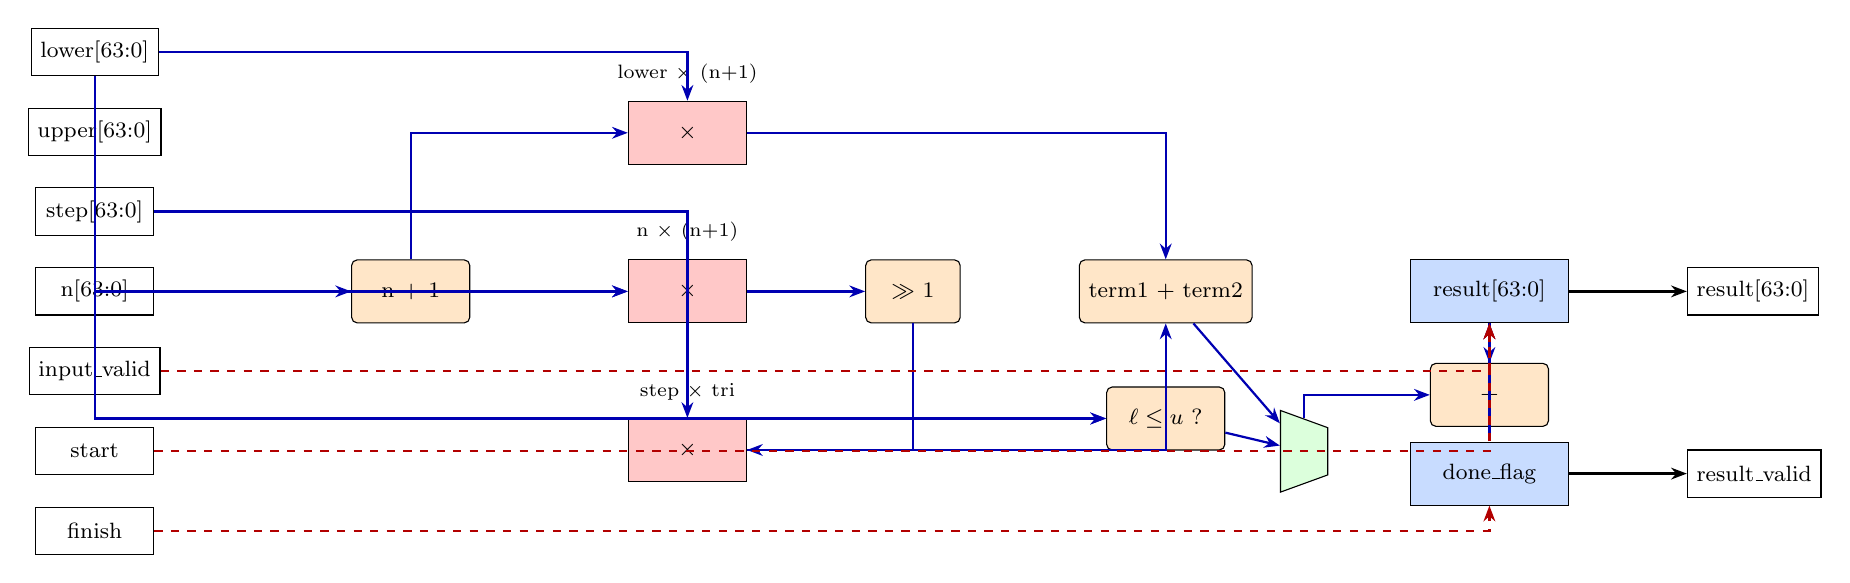
\begin{tikzpicture}[node distance=1.2cm and 1.8cm]

% Input ports
\node[io] (lower) {lower[63:0]};
\node[io, below=0.4cm of lower] (upper) {upper[63:0]};
\node[io, below=0.4cm of upper] (step) {step[63:0]};
\node[io, below=0.4cm of step] (nval) {n[63:0]};
\node[io, below=0.4cm of nval] (valid) {input\_valid};
\node[io, below=0.4cm of valid] (start) {start};
\node[io, below=0.4cm of start] (finish) {finish};

% n+1 adder
\node[comblogic, right=2.5cm of nval, minimum width=1.5cm] (nplus1) {n + 1};

% Multipliers
\node[mult, right=2cm of nplus1] (mult1) {$\times$};
\node[mult, above=1.2cm of mult1] (mult2) {$\times$};
\node[mult, below=1.2cm of mult1] (mult3) {$\times$};

% Labels for multipliers
\node[above=0.1cm of mult2, font=\scriptsize] {lower $\times$ (n+1)};
\node[above=0.1cm of mult1, font=\scriptsize] {n $\times$ (n+1)};
\node[above=0.1cm of mult3, font=\scriptsize] {step $\times$ tri};

% Right shift
\node[comblogic, right=1.5cm of mult1, minimum width=1.2cm] (shr) {$\gg$ 1};

% Final adder
\node[comblogic, right=1.5cm of shr, minimum width=1.5cm] (adder) {term1 + term2};

% Valid check
\node[comblogic, below=0.8cm of adder, minimum width=1.5cm] (validchk) {$\ell \leq u$ ?};

% Mux for valid
\node[mux, right=1cm of validchk, rotate=-90] (valmux) {};

% Accumulator
\node[register, right=2cm of adder] (acc) {result[63:0]};
\node[comblogic, below=0.5cm of acc, minimum width=1.5cm] (accadd) {+};

% Done flag
\node[register, below=1.5cm of acc] (done) {done\_flag};

% Output ports
\node[io, right=1.5cm of acc] (outres) {result[63:0]};
\node[io, right=1.5cm of done] (outvalid) {result\_valid};

% Data flow arrows
\draw[dataarrow] (nval) -- (nplus1);
\draw[dataarrow] (nplus1) -- (mult1);
\draw[dataarrow] (nval) |- (mult1);
\draw[dataarrow] (lower) -| (mult2);
\draw[dataarrow] (nplus1) |- (mult2);
\draw[dataarrow] (mult1) -- (shr);
\draw[dataarrow] (step) -| (mult3);
\draw[dataarrow] (shr) |- (mult3);
\draw[dataarrow] (mult2) -| (adder);
\draw[dataarrow] (mult3) -| (adder);
\draw[dataarrow] (adder) -- (valmux);
\draw[dataarrow] (lower) |- (validchk);
\draw[dataarrow] (upper) |- (validchk);
\draw[dataarrow] (validchk) -- (valmux);
\draw[dataarrow] (valmux) |- (accadd);
\draw[dataarrow] (acc) -- (accadd);
\draw[dataarrow] (accadd) -- ++(0,-0.5) -| (acc);

% Control arrows
\draw[ctrlarrow] (valid) -| (acc);
\draw[ctrlarrow] (start) -| (acc);
\draw[ctrlarrow] (finish) -| (done);

% Outputs
\draw[arrow] (acc) -- (outres);
\draw[arrow] (done) -- (outvalid);

\end{tikzpicture}
\caption{Gift Shop sum accumulator circuit}
\end{figure}

\section{Key Components}

\subsection{Arithmetic Sum Unit}

The core computation implements the closed-form sum formula:
\begin{equation}
    \text{pair\_sum} = \underbrace{\ell \cdot (n+1)}_{\text{term1}} + \underbrace{s \cdot \frac{n(n+1)}{2}}_{\text{term2}}
\end{equation}

Three 64-bit multipliers compute the products. The division by 2 is a simple right shift by one bit. All operations are purely combinational.

\subsection{Width Management}

64-bit multiplication produces 128-bit results. Since the problem guarantees results fit in 64 bits, we truncate intermediate products using \texttt{sel\_bottom}:

\begin{lstlisting}[basicstyle=\ttfamily\small]
let term1 = sel_bottom (lower *: n_plus_1) ~width:64
let n_times_np1 = sel_bottom (n *: n_plus_1) ~width:64
let triangular = srl n_times_np1 ~by:1
let term2 = sel_bottom (step *: triangular) ~width:64
\end{lstlisting}

\subsection{Validity Check}

If the intersection is empty ($\ell > u$), the mux outputs zero instead of the computed sum. This handles cases where a pattern doesn't overlap with the input range.

\subsection{Accumulator}

A single 64-bit register accumulates sums across all (pattern, range) pairs. The \texttt{start} signal resets it to zero; each \texttt{input\_valid} pulse adds the current pair's sum.

\section{Performance}

The circuit processes one (pattern, range) pair per clock cycle. For part 1 with 5 patterns and 32 ranges, that's $5 \times 32 = 160$ cycles. Part 2 requires three simulation runs (part1 patterns, extra patterns, overlaps to subtract), totaling under 500 cycles for the complete solution.

\section{Testbench Precomputation}

Pattern parameters are derived from digit count $d$ and block size $b$:
\begin{align}
    \text{step} &= \frac{10^d - 1}{10^b - 1} \\
    \text{start} &= \text{step} \times \frac{10^b}{10} \\
    \text{end} &= \text{step} \times (10^b - 1)
\end{align}

For example, 4-digit patterns with 2-digit blocks: step = 9999/99 = 101, start = 101 $\times$ 10 = 1010, end = 101 $\times$ 99 = 9999.

\section{Part 2 Inclusion-Exclusion}

Part 2 counts IDs where patterns repeat at least twice. This requires inclusion-exclusion to avoid double-counting:
\begin{equation}
    \text{part2} = \text{part1} + \text{extra\_patterns} - \text{overlaps}
\end{equation}

where overlaps are patterns like ``all same digit'' (111, 222222) that match multiple block sizes.

\end{document}
